\section{Convolutional Neural Networks Overview}
Convolutional Neural Networks (CNN's) are essentially a Multi Layered Perceptron with a
special structure. CNN's have one major difference from a MLP, they have extra
layers of convolution and pooling. The architecture of a convolution network can
be seen in Figure \ref{fig:convNet}.

\begin{figure}[h]
	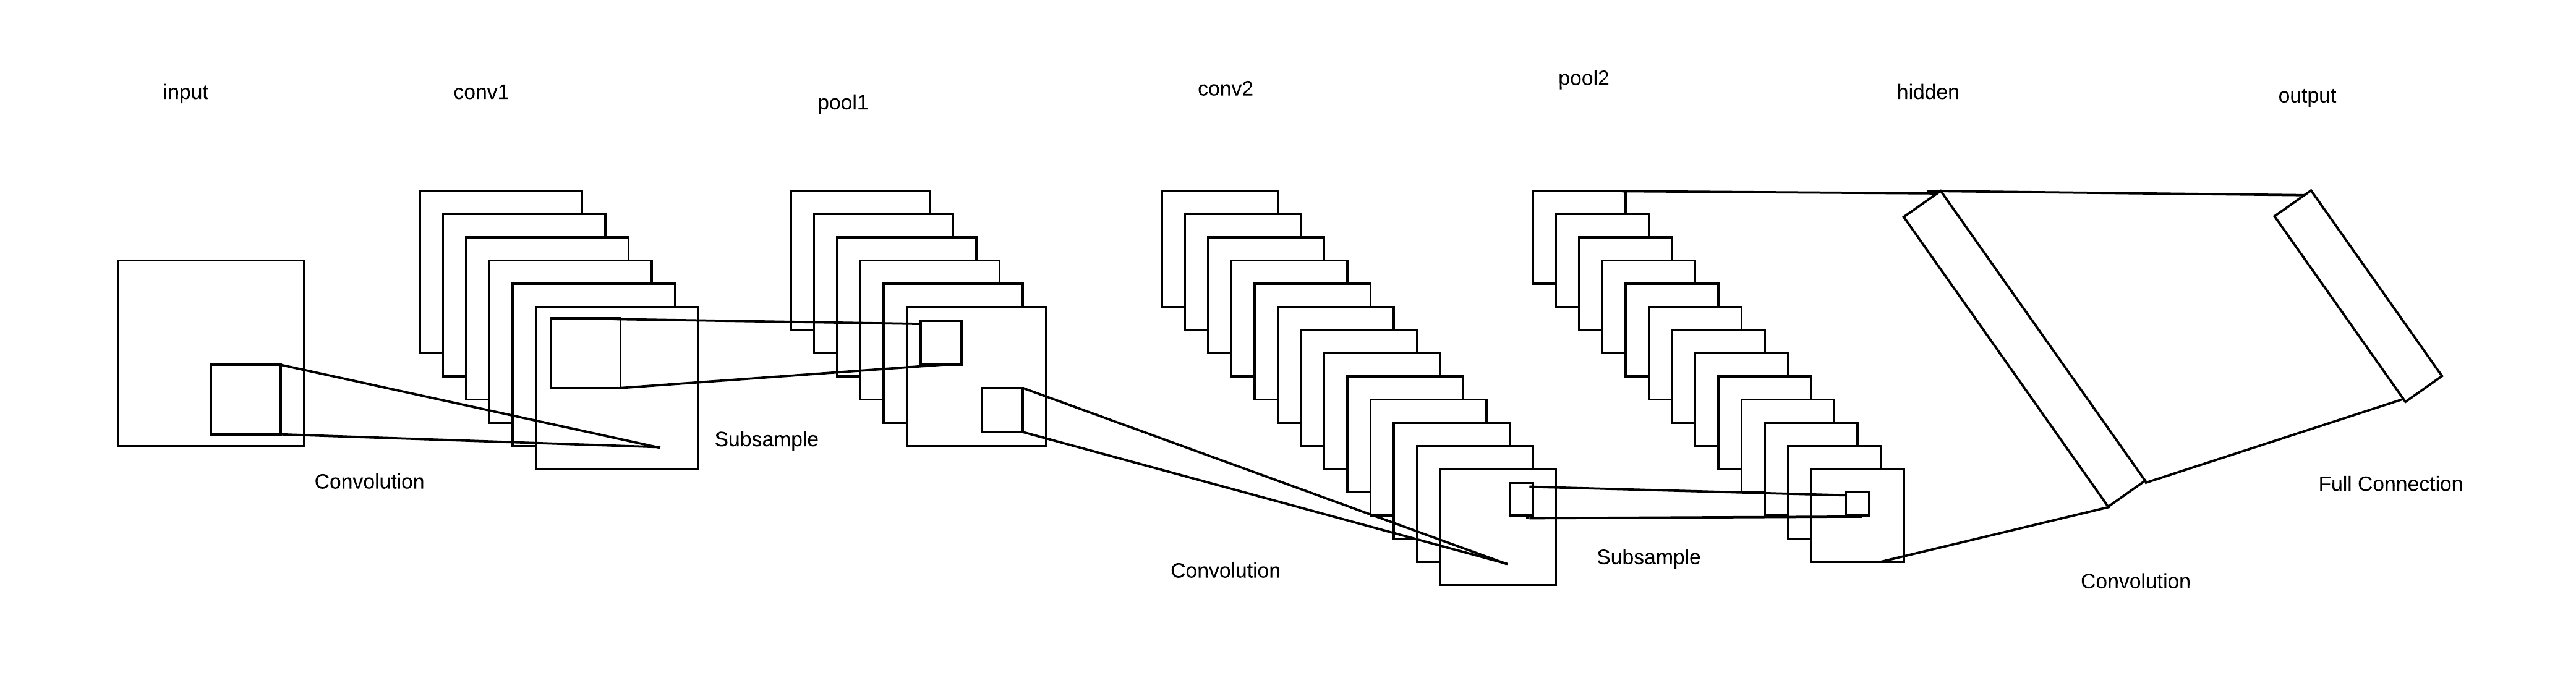
\includegraphics[width=150mm, scale=0.5]{convNet}
	\caption{CNN Architecture}
	\label{fig:convNet}
\end{figure}

Figure \ref{fig:cnnExplain} (a) shows an image that we want to compare against
Figure \ref{fig:cnnExplain} (b).
For humans, it is quite easy to determine that these images are very similar but
for a computer this task is surprisingly difficult.

So what a CNN does, to combat this problem, is to take a small feature from
Figure \ref{fig:cnnExplain} (a) and compare it to a subsection of Figure \ref{fig:cnnExplain} (b).
The CNN multiplies the feature and a section of Figure \ref{fig:cnnExplain} (c), adds
up the results and divides by 9 (The number of pixels in the feature). This then gives a decimal value of how likely
it is that the feature is in the part of the image, as seen in Figure
\ref{fig:cnnExplain} (d).
This is called filtering. The Convolutional layer is composed of carrying out
this filtering for every single possible location in Figure \ref{fig:cnnExplain} (a).

\begin{figure}
    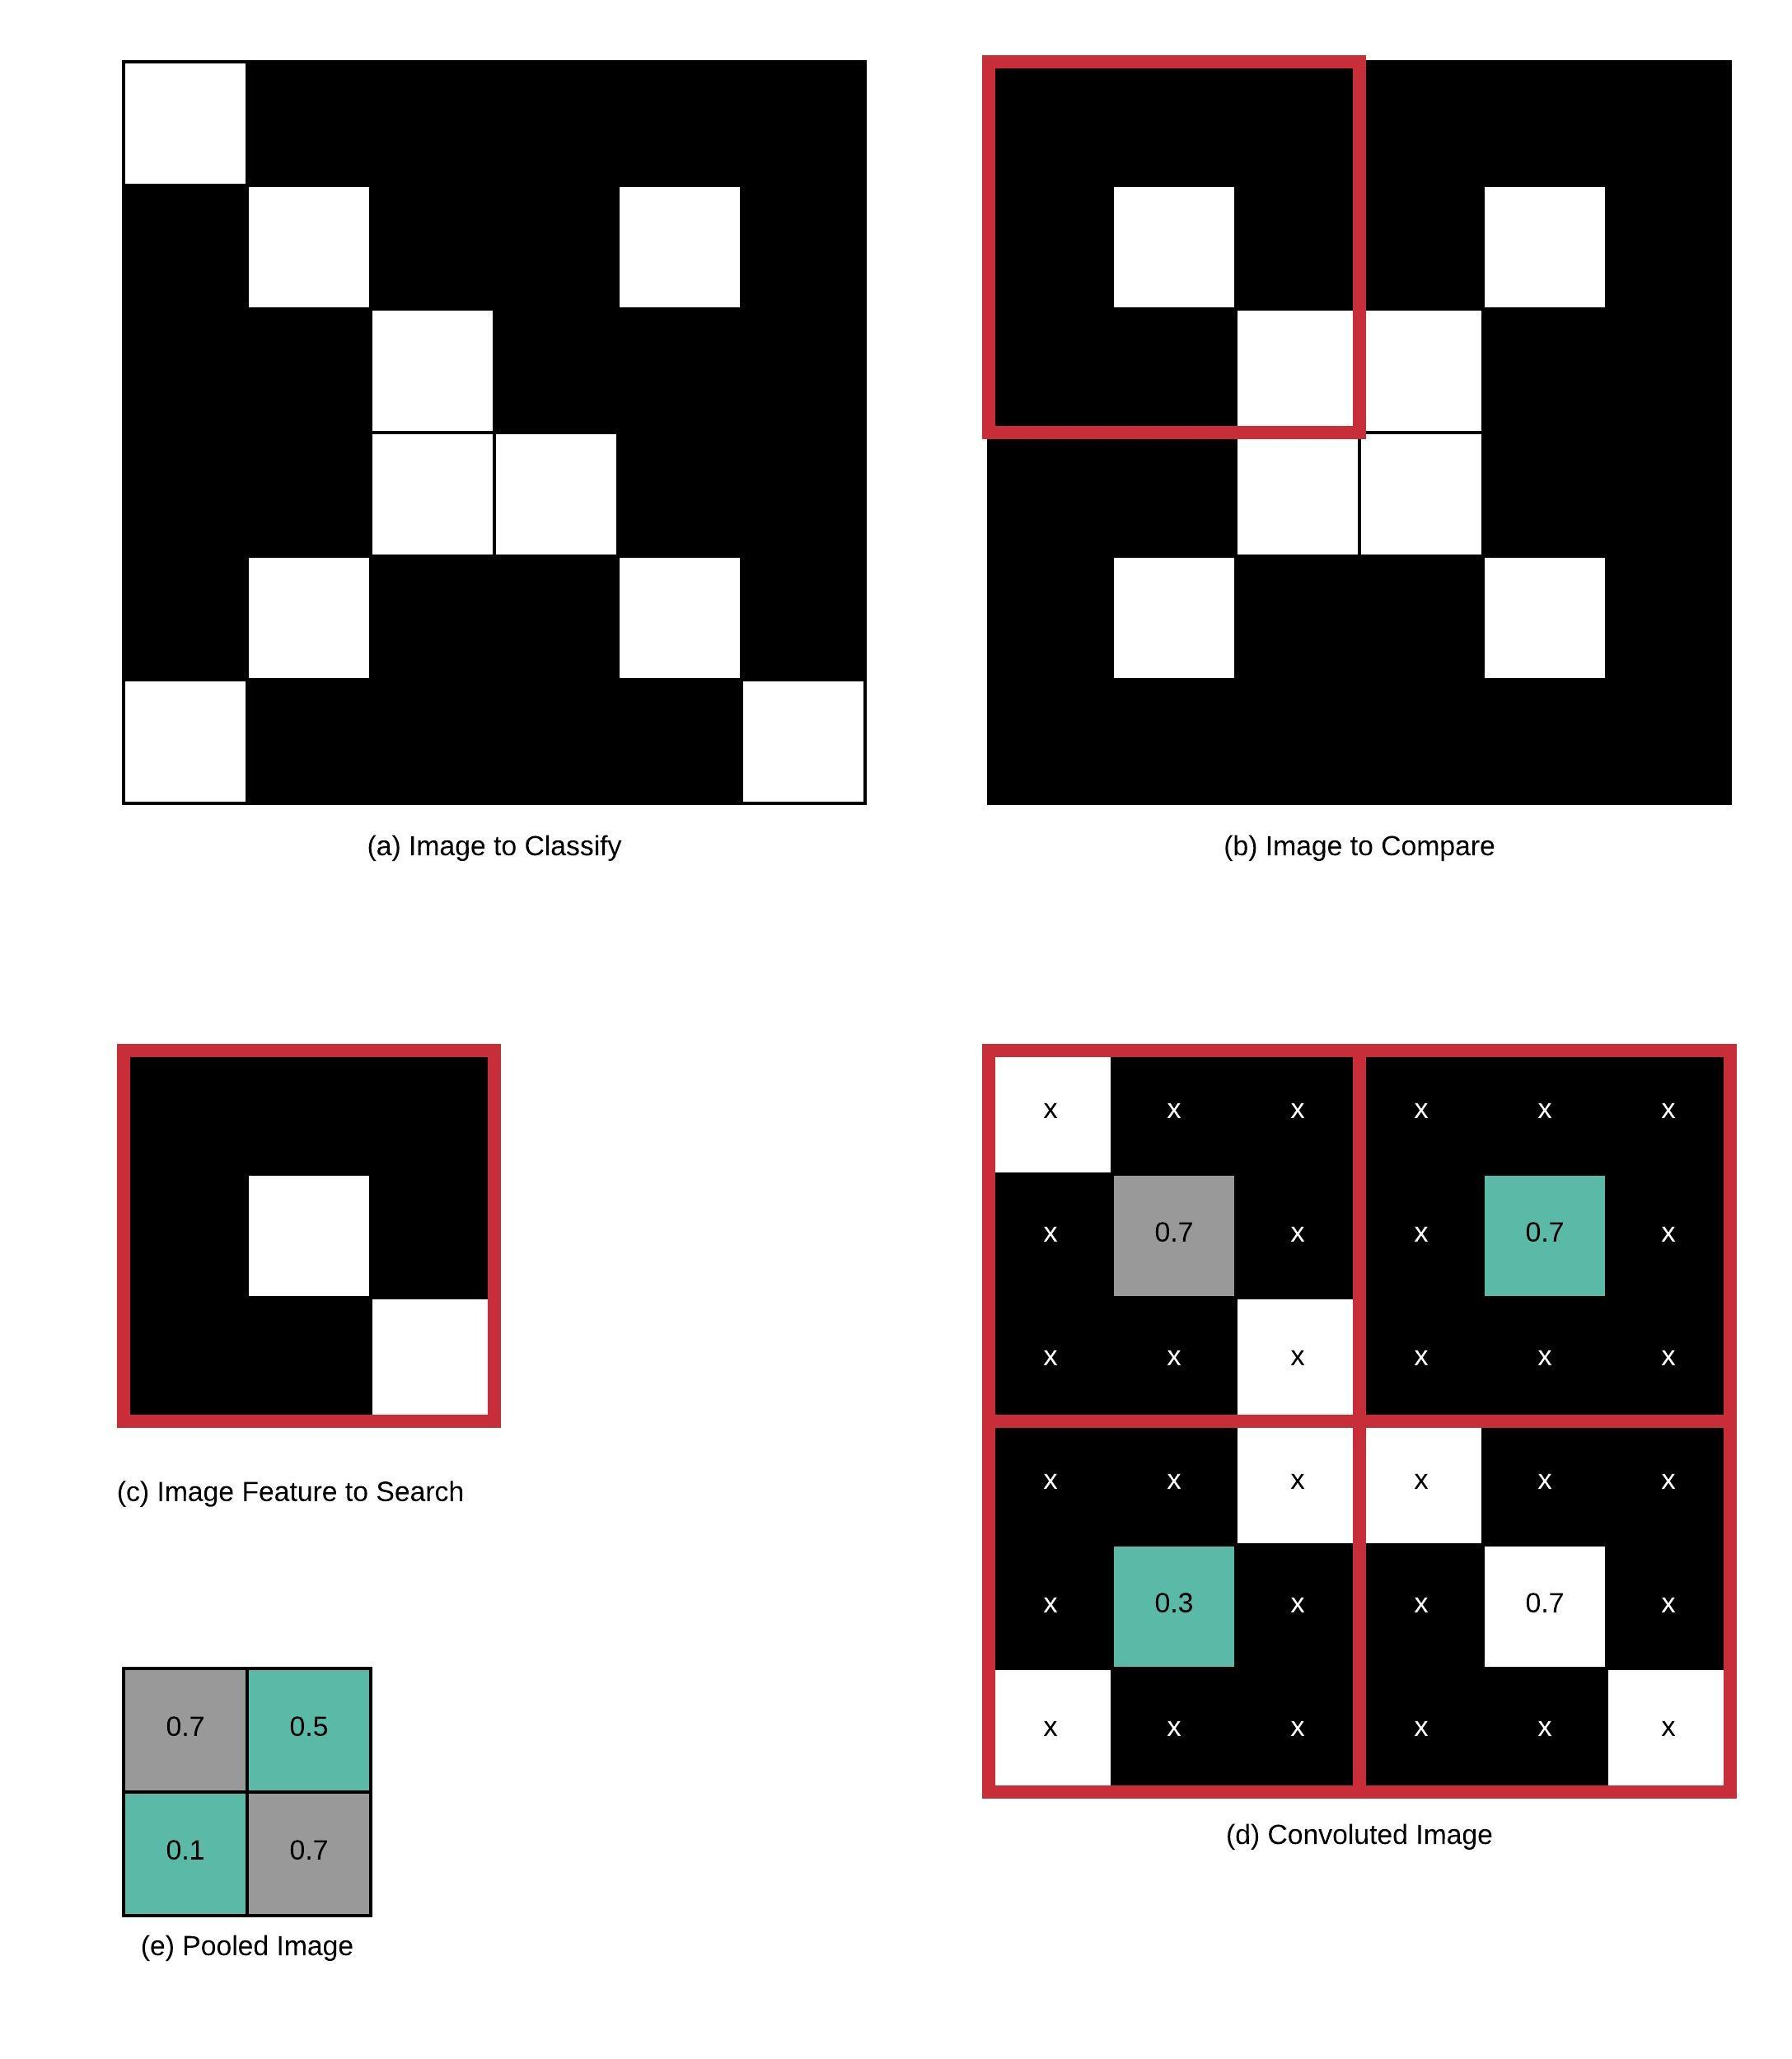
\includegraphics[scale=0.75]{cnnExplain}
    \caption{CNN Overview}
    \label{fig:cnnExplain}
\end{figure}
Next is the Pooling Layer, this layer takes the convoluted
layer output (you can use Figure \ref{fig:cnnExplain} (d) as reference) and from a
user defined size ie. 2x2, gets either the highest decimal value (Max pooling)
, the average value (Mean pooling) or the lowest decimal value (Min pooling) and records that as the new value for the
section. This is then applied to the entire image. As we can see in Figure
\ref{fig:cnnExplain} (e) we now have a much smaller image stack in which to classify,
thus making the computation easier. Pooling also makes features of the image clearer which helps to result in more accurate classification.

In between the Convolution and Pooling layer, there is sometimes a Normalization
layer. This Normalization layer creates Rectified Linear Units (RLU's). In other
words, if we take Figure \ref{fig:cnnExplain} (d), it changes all minus values to
zero.

There are some problems with CNN's however. One of the main problems is that you
need a very large dataset in order to produce am accurate model and the training
can be very time consuming without a GPU.